\documentclass{article}\usepackage[]{graphicx}\usepackage[]{color}
%% maxwidth is the original width if it is less than linewidth
%% otherwise use linewidth (to make sure the graphics do not exceed the margin)
\makeatletter
\def\maxwidth{ %
  \ifdim\Gin@nat@width>\linewidth
    \linewidth
  \else
    \Gin@nat@width
  \fi
}
\makeatother

\definecolor{fgcolor}{rgb}{0.345, 0.345, 0.345}
\newcommand{\hlnum}[1]{\textcolor[rgb]{0.686,0.059,0.569}{#1}}%
\newcommand{\hlstr}[1]{\textcolor[rgb]{0.192,0.494,0.8}{#1}}%
\newcommand{\hlcom}[1]{\textcolor[rgb]{0.678,0.584,0.686}{\textit{#1}}}%
\newcommand{\hlopt}[1]{\textcolor[rgb]{0,0,0}{#1}}%
\newcommand{\hlstd}[1]{\textcolor[rgb]{0.345,0.345,0.345}{#1}}%
\newcommand{\hlkwa}[1]{\textcolor[rgb]{0.161,0.373,0.58}{\textbf{#1}}}%
\newcommand{\hlkwb}[1]{\textcolor[rgb]{0.69,0.353,0.396}{#1}}%
\newcommand{\hlkwc}[1]{\textcolor[rgb]{0.333,0.667,0.333}{#1}}%
\newcommand{\hlkwd}[1]{\textcolor[rgb]{0.737,0.353,0.396}{\textbf{#1}}}%

\usepackage{framed}
\makeatletter
\newenvironment{kframe}{%
 \def\at@end@of@kframe{}%
 \ifinner\ifhmode%
  \def\at@end@of@kframe{\end{minipage}}%
  \begin{minipage}{\columnwidth}%
 \fi\fi%
 \def\FrameCommand##1{\hskip\@totalleftmargin \hskip-\fboxsep
 \colorbox{shadecolor}{##1}\hskip-\fboxsep
     % There is no \\@totalrightmargin, so:
     \hskip-\linewidth \hskip-\@totalleftmargin \hskip\columnwidth}%
 \MakeFramed {\advance\hsize-\width
   \@totalleftmargin\z@ \linewidth\hsize
   \@setminipage}}%
 {\par\unskip\endMakeFramed%
 \at@end@of@kframe}
\makeatother

\definecolor{shadecolor}{rgb}{.97, .97, .97}
\definecolor{messagecolor}{rgb}{0, 0, 0}
\definecolor{warningcolor}{rgb}{1, 0, 1}
\definecolor{errorcolor}{rgb}{1, 0, 0}
\newenvironment{knitrout}{}{} % an empty environment to be redefined in TeX

\usepackage{alltt}
\usepackage[T1]{fontenc}
\usepackage{geometry}
\geometry{verbose,tmargin=2.5cm,bmargin=2.5cm,lmargin=2.5cm,rmargin=2.5cm}
\setcounter{secnumdepth}{2}
\setcounter{tocdepth}{2}
\usepackage{url}
\usepackage{verbatim}
\usepackage[unicode=true,pdfusetitle,
 bookmarks=true,bookmarksnumbered=true,bookmarksopen=true,bookmarksopenlevel=2,
 breaklinks=false,pdfborder={0 0 1},backref=false,colorlinks=false]
 {hyperref}
\usepackage{breakurl}
\hypersetup{pdfborder = {0 0 0 0}}
\IfFileExists{upquote.sty}{\usepackage{upquote}}{}
\begin{document}





\title{A Minimal Demo of knitr}


\author{Yihui Xie}

\maketitle
You can test if \textbf{knitr} works with this minimal demo. OK, let's
get started with some boring random numbers:

\begin{knitrout}
\definecolor{shadecolor}{rgb}{0.969, 0.969, 0.969}\color{fgcolor}\begin{kframe}
\begin{alltt}
\hlkwd{set.seed}\hlstd{(}\hlnum{1121}\hlstd{)}
\hlstd{(x} \hlkwb{<-} \hlkwd{rnorm}\hlstd{(}\hlnum{20}\hlstd{))}
\end{alltt}
\begin{verbatim}
##  [1]  0.14496  0.43832  0.15319  1.08494  1.99954 -0.81188  0.16027  0.58589  0.36009
## [10] -0.02531  0.15088  0.11008  1.35968 -0.32699 -0.71638  1.80977  0.50840 -0.52746
## [19]  0.13272 -0.15594
\end{verbatim}
\begin{alltt}
\hlkwd{mean}\hlstd{(x)}
\end{alltt}
\begin{verbatim}
## [1] 0.3217
\end{verbatim}
\begin{alltt}
\hlkwd{var}\hlstd{(x)}
\end{alltt}
\begin{verbatim}
## [1] 0.5715
\end{verbatim}
\end{kframe}
\end{knitrout}


\clearpage
\section{Your Turn 1}

\begin{knitrout}
\definecolor{shadecolor}{rgb}{0.969, 0.969, 0.969}\color{fgcolor}\begin{kframe}
\begin{alltt}
\hlkwd{set.seed}\hlstd{(}\hlnum{1121}\hlstd{)}
\hlstd{(x} \hlkwb{<-} \hlkwd{rnorm}\hlstd{(}\hlnum{30}\hlstd{))}
\end{alltt}
\begin{verbatim}
##  [1]  0.14496  0.43832  0.15319  1.08494  1.99954 -0.81188  0.16027  0.58589  0.36009
## [10] -0.02531  0.15088  0.11008  1.35968 -0.32699 -0.71638  1.80977  0.50840 -0.52746
## [19]  0.13272 -0.15594  0.06415 -0.07236  0.08807  0.29775 -0.66460 -1.15103  0.40493
## [28] -0.46179 -0.79187  0.08349
\end{verbatim}
\begin{alltt}
\hlkwd{sum}\hlstd{(x)}
\end{alltt}
\begin{verbatim}
## [1] 4.232
\end{verbatim}
\begin{alltt}
\hlkwd{mean}\hlstd{(x)}
\end{alltt}
\begin{verbatim}
## [1] 0.1411
\end{verbatim}
\begin{alltt}
\hlkwd{var}\hlstd{(x)}
\end{alltt}
\begin{verbatim}
## [1] 0.5246
\end{verbatim}
\end{kframe}
\end{knitrout}

\clearpage
\section{Your Turn 2}

\begin{knitrout}
\definecolor{shadecolor}{rgb}{0.969, 0.969, 0.969}\color{fgcolor}\begin{kframe}
\begin{alltt}
\hlkwd{set.seed}\hlstd{(}\hlnum{1121}\hlstd{)}

\hlstd{x} \hlkwb{<-} \hlkwd{rnorm}\hlstd{(}\hlnum{50}\hlstd{)}

\hlkwd{library}\hlstd{(ggplot2)}
\hlkwd{qplot}\hlstd{(x,} \hlkwc{geom} \hlstd{=} \hlstr{"histogram"}\hlstd{)}
\end{alltt}


{\ttfamily\noindent\itshape\color{messagecolor}{\#\# stat\_bin: binwidth defaulted to range/30. Use 'binwidth = x' to adjust this.}}\end{kframe}

{\centering 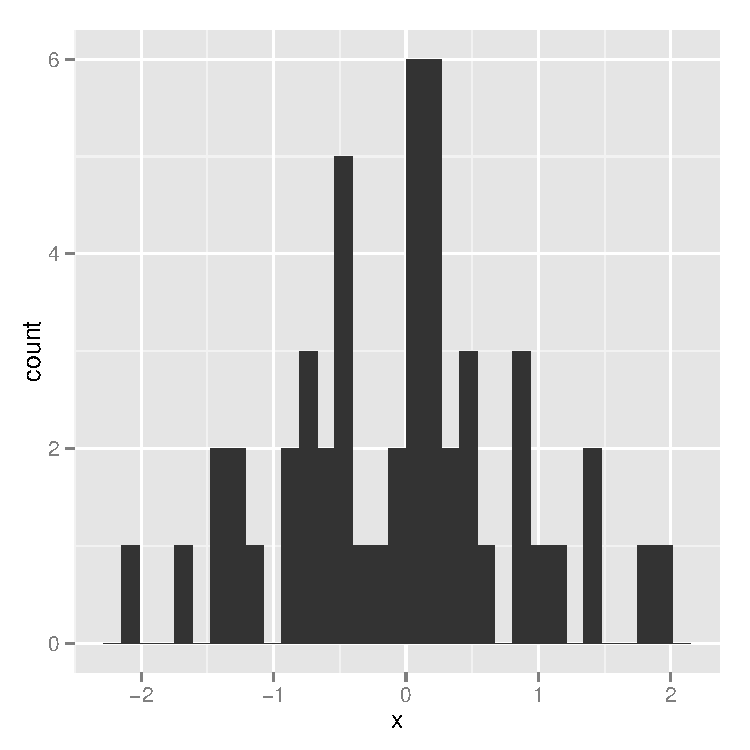
\includegraphics[width=\textwidth]{figure/pretty-histogram1} 

}



\end{knitrout}

\clearpage
\section{Your Turn 3}
\noindent Knitr options: message=FALSE, warning=FALSE
\begin{knitrout}
\definecolor{shadecolor}{rgb}{0.969, 0.969, 0.969}\color{fgcolor}\begin{kframe}
\begin{alltt}
\hlkwd{set.seed}\hlstd{(}\hlnum{1121}\hlstd{)}
\hlstd{x} \hlkwb{<-} \hlkwd{rnorm}\hlstd{(}\hlnum{50}\hlstd{)}
\hlkwd{library}\hlstd{(ggplot2)}
\hlkwd{qplot}\hlstd{(x,} \hlkwc{geom} \hlstd{=} \hlstr{"histogram"}\hlstd{)}
\end{alltt}
\end{kframe}

{\centering 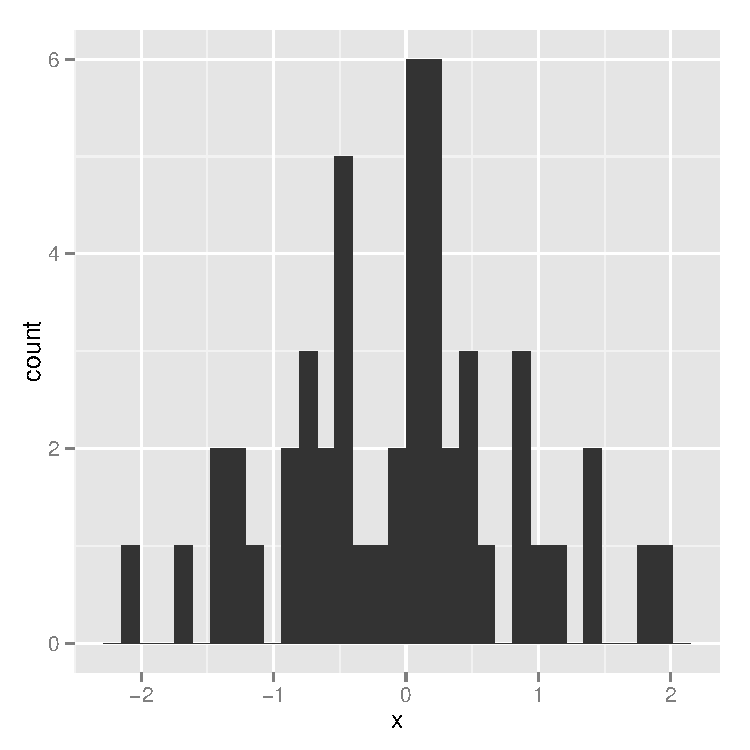
\includegraphics[width=\textwidth]{figure/pretty-histogram2} 

}



\end{knitrout}


\clearpage
\noindent Knitr options: message=FALSE, tidy=FALSE\\
Note that the spacing of the code is different than on the previous page.
\begin{knitrout}
\definecolor{shadecolor}{rgb}{0.969, 0.969, 0.969}\color{fgcolor}\begin{kframe}
\begin{alltt}
\hlkwd{set.seed}\hlstd{(}\hlnum{1121}\hlstd{)}
\hlstd{x}\hlkwb{<-}\hlkwd{rnorm}\hlstd{(}\hlnum{50}\hlstd{)}
\hlkwd{library}\hlstd{(ggplot2)}
\hlkwd{qplot}\hlstd{(x,}\hlkwc{geom}\hlstd{=}\hlstr{"histogram"}\hlstd{)}
\end{alltt}
\end{kframe}

{\centering 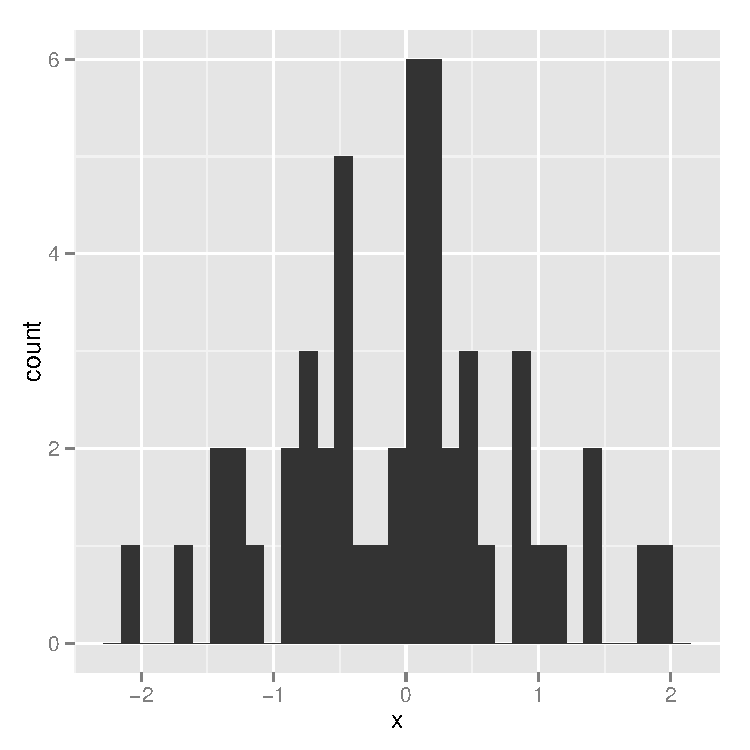
\includegraphics[width=\textwidth]{figure/pretty-histogram3} 

}



\end{knitrout}


\clearpage
\noindent Knitr options: dependson='pretty-histogram1', message=FALSE, echo=FALSE\\
I'm using the previously generated $x$, not re-generating it.\\
Note that now only the plot shows up.
\begin{knitrout}
\definecolor{shadecolor}{rgb}{0.969, 0.969, 0.969}\color{fgcolor}

{\centering 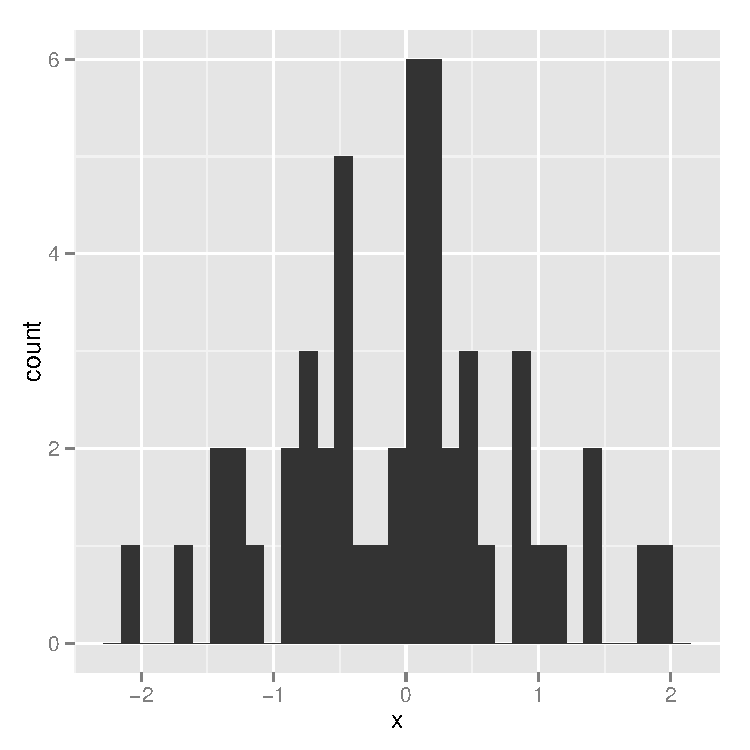
\includegraphics[width=\textwidth]{figure/pretty-histogram4} 

}



\end{knitrout}


\clearpage
\section{Your Turn 4}
\noindent Knitr options: dependson='pretty-histogram1', message=FALSE, out.width='.49\textbackslash\textbackslash textwidth'
\begin{knitrout}
\definecolor{shadecolor}{rgb}{0.969, 0.969, 0.969}\color{fgcolor}\begin{kframe}
\begin{alltt}
\hlkwd{qplot}\hlstd{(x,} \hlkwc{geom} \hlstd{=} \hlstr{"histogram"}\hlstd{)}
\end{alltt}
\end{kframe}

{\centering 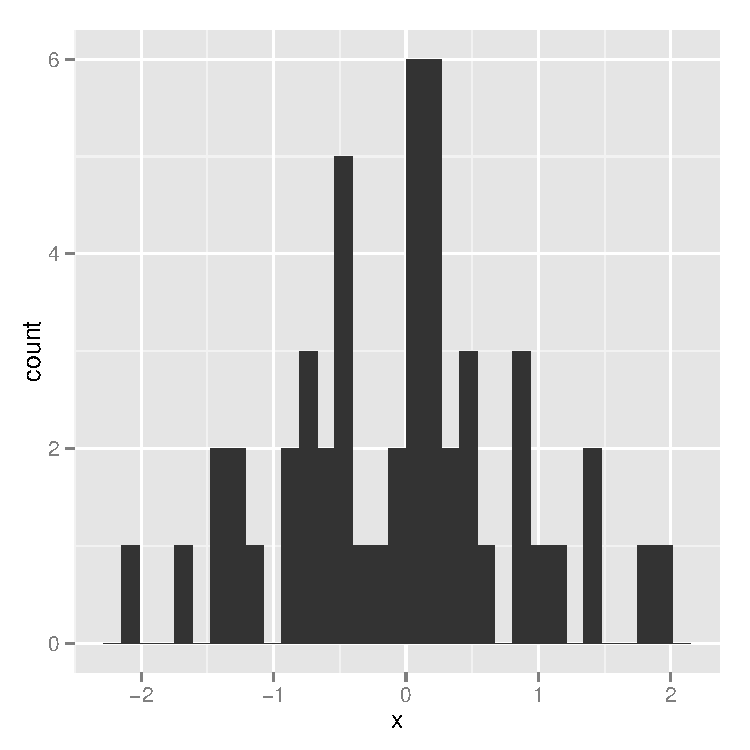
\includegraphics[width=.49\textwidth]{figure/lots-of-plots1} 

}


\begin{kframe}\begin{alltt}
\hlkwd{qplot}\hlstd{(x,} \hlkwc{geom} \hlstd{=} \hlstr{"density"}\hlstd{)}
\end{alltt}
\end{kframe}

{\centering 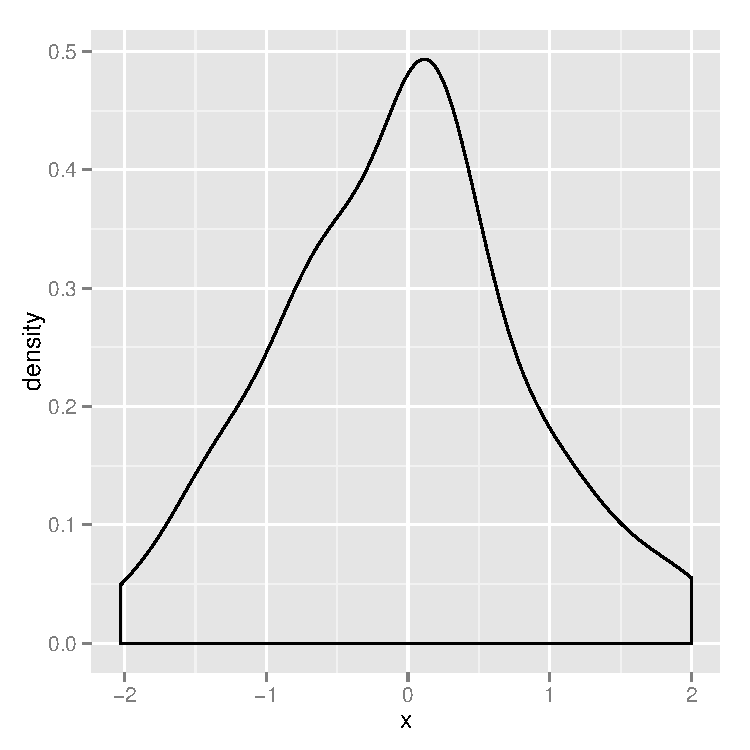
\includegraphics[width=.49\textwidth]{figure/lots-of-plots2} 

}



\end{knitrout}

\hrule\vspace{12pt}
\noindent Knitr options: dependson='pretty-histogram1', message=FALSE, out.width='.49\textbackslash\textbackslash textwidth', fig.show='hide'
\begin{knitrout}
\definecolor{shadecolor}{rgb}{0.969, 0.969, 0.969}\color{fgcolor}\begin{kframe}
\begin{alltt}
\hlkwd{qplot}\hlstd{(x,} \hlkwc{geom} \hlstd{=} \hlstr{"histogram"}\hlstd{)}
\hlkwd{qplot}\hlstd{(x,} \hlkwc{geom} \hlstd{=} \hlstr{"density"}\hlstd{)}
\end{alltt}
\end{kframe}
\end{knitrout}

\hrule\vspace{12pt}
\noindent Knitr options: dependson='pretty-histogram1', message=FALSE, out.width='.49\textbackslash\textbackslash textwidth', fig.show='hold'

\begin{knitrout}
\definecolor{shadecolor}{rgb}{0.969, 0.969, 0.969}\color{fgcolor}\begin{kframe}
\begin{alltt}
\hlkwd{qplot}\hlstd{(x,} \hlkwc{geom} \hlstd{=} \hlstr{"histogram"}\hlstd{)}
\hlkwd{qplot}\hlstd{(x,} \hlkwc{geom} \hlstd{=} \hlstr{"density"}\hlstd{)}
\end{alltt}
\end{kframe}

{\centering 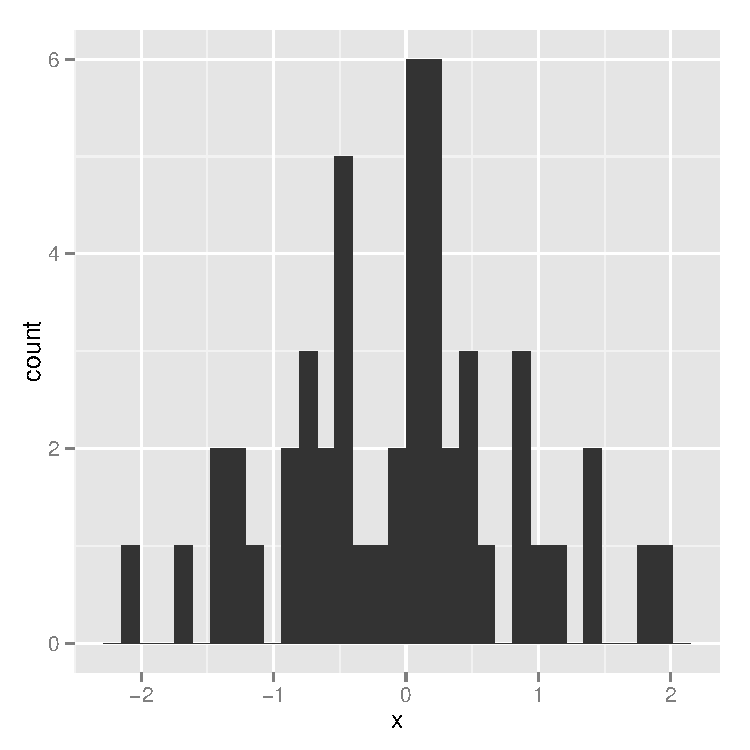
\includegraphics[width=.49\textwidth]{figure/lots-of-plots31} 
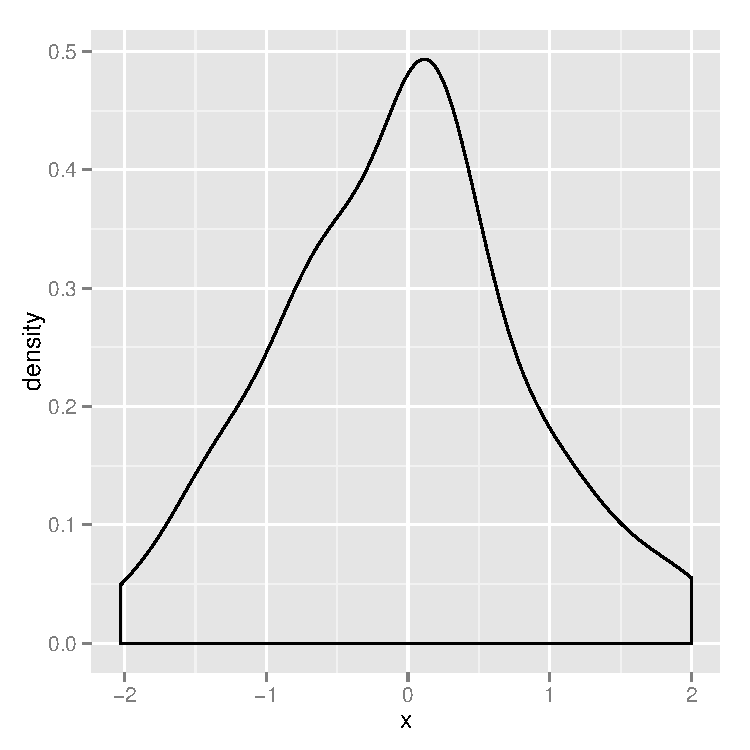
\includegraphics[width=.49\textwidth]{figure/lots-of-plots32} 

}



\end{knitrout}


\hrule\vspace{12pt}
\noindent Knitr options: dependson='pretty-histogram1', message=FALSE, out.width='.49\textbackslash\textbackslash textwidth', fig.keep='last'

\begin{knitrout}
\definecolor{shadecolor}{rgb}{0.969, 0.969, 0.969}\color{fgcolor}\begin{kframe}
\begin{alltt}
\hlkwd{qplot}\hlstd{(x,} \hlkwc{geom} \hlstd{=} \hlstr{"histogram"}\hlstd{)}
\hlkwd{qplot}\hlstd{(x,} \hlkwc{geom} \hlstd{=} \hlstr{"density"}\hlstd{)}
\end{alltt}
\end{kframe}

{\centering 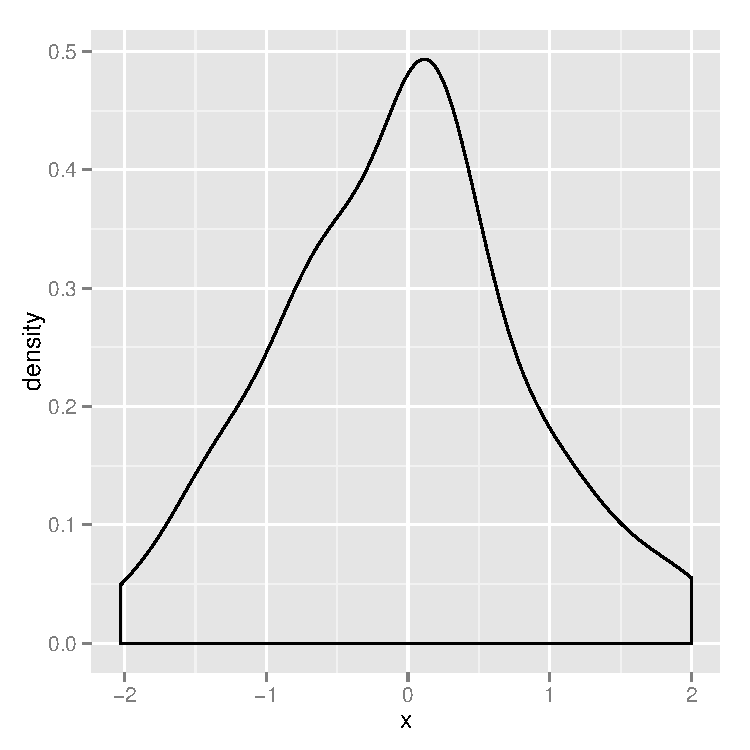
\includegraphics[width=.49\textwidth]{figure/lots-of-plots4} 

}



\end{knitrout}


\clearpage
\hrule\vspace{12pt}
\noindent Including pictures directly: code chunk options - include=FALSE




\begin{figure}[h!]
\centering
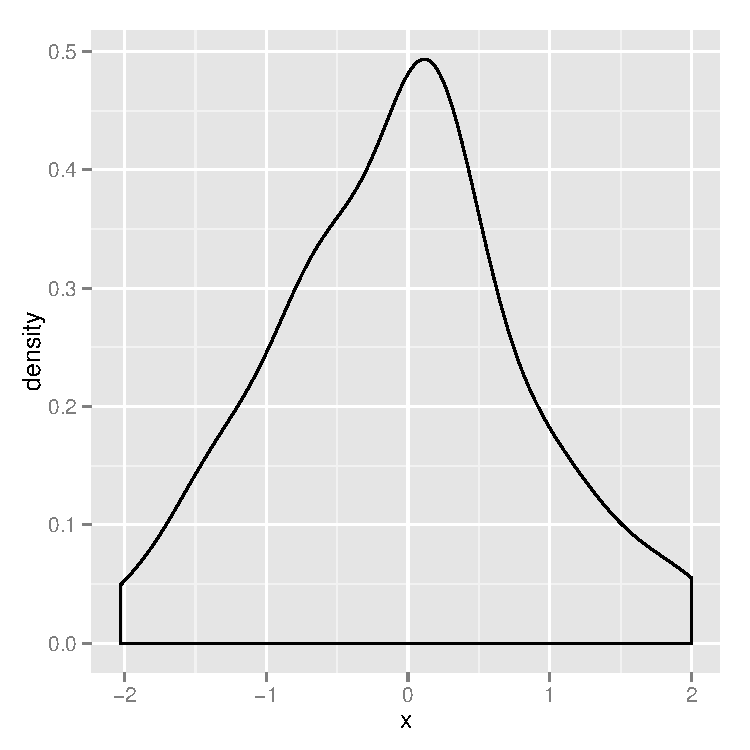
\includegraphics[keepaspectratio=TRUE,width=.5\textwidth]{figure/lots-of-plots5}
\caption{What a nice figure}
\end{figure}

\noindent Do this by using 
\begin{verbatim}
\begin{figure}[h!]
\centering
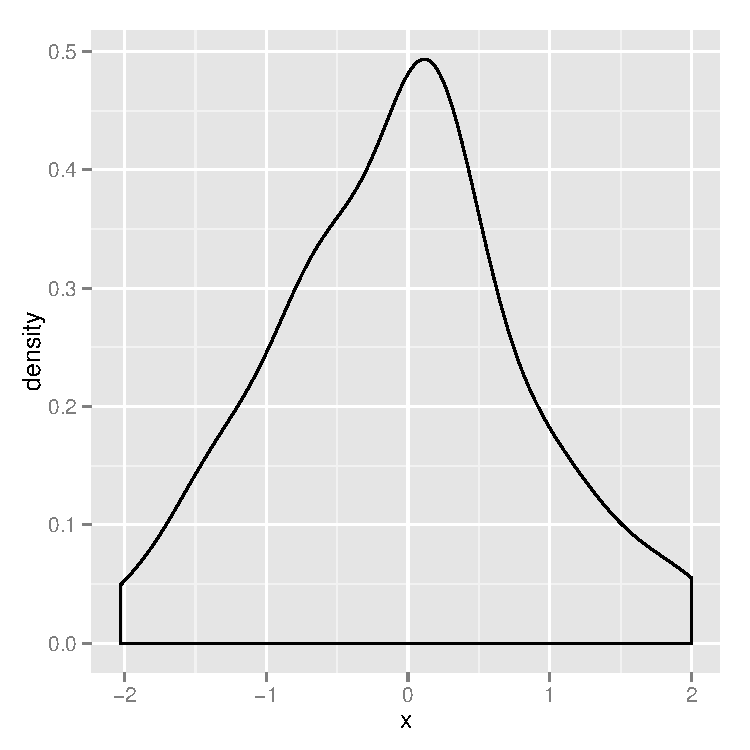
\includegraphics[keepaspectratio=TRUE,width=.5\textwidth]{figure/lots-of-plots5}
\caption{What a nice figure}
\end{figure}
\end{verbatim}

\end{document}
